\chapter{Installation and Configuration}

\section{Software requirements}

The \fmipp \trnsys FMU Export Utility is intended to run on Windows~7~(32-bit).

The following applications need to be installed prior to installing the \fmipp \trnsys FMU Export Utility:
\begin{itemize}

  \item \href{http://www.trnsys.com/}{\trnsys~17}

  \item For creating FMUs from command line \href{https://www.python.org/}{\python} (tested with \python~3.5) is required.

  \item For compiling FMUs according to FMI version 1.0 a version of Microsoft Visual Studio Express 2013 for Windows Desktop has to be installed.
\end{itemize}

\textbf{Note}: An installed version of \trnsys (and Simulation Studio) is necessary to create deck files and to use the generated FMUs in a simulation. It is not required to generated an FMU from a deck file.

\textbf{Note}: For generating FMUs with the help of the graphical user interface \python is not required.

\textbf{Note}: For generating FMUs according to FMI version 2.0 (default) Microsoft Visual Studio Express 2013 for Windows Desktop is not required.


\section{Installation}
\label{sec:install}

To install the \fmipp \trnsys FMU Export Utility, proceed as follows:
\begin{itemize}

  \item Download the latest version as ZIP-file from the \href{http://sourceforge.net/projects/trnsys-fmu/files/latest/download}{download page}.

  \item Unzip the installation file into any sub directory (referred to as the \emph{installation directory}).

  \item Switch to the installation directory and start program \texttt{trnsys\_fmu\_install.exe} (double-click).
  This should bring up the window shown in Figure~\ref{fig:trnsys_fmu_install_gui}.

  \item Provide the path to the TRNSYS installation directory and press \textit{Start}.

\end{itemize}

After successful installation, \type is available in the \trnsys Simulation Studio. An additional directory called \emph{FMI} should be available in the toolbar on the right-hand side, containing the new \trnsys type (\emph{\typea} and \emph{\typeb}), see Figure~\ref{fig:simulation_studio_overview} for a snapshot.


\section{Installation using a Python script}
\label{sec:install_script}

Alternatively, the installation can be done by running a Python script.
This requires to execute \python from the command prompt window, please refer to the \href{https://docs.python.org/2/faq/windows.html}{\python~FAQ} in case you need assistance with this.
Open the command prompt window, change to the installation directory and execute the script \texttt{trnsys\_fmu\_install.py}:
\begin{verbatim}
python.exe trnsys_fmu_install.py <trnsys_install_dir>
\end{verbatim}
where \texttt{<trnsys\_install\_dir>} is the path to your local \trnsys installation directory (typically \texttt{C:\symbol{92}Trnsys17}).

\begin{figure}[h]
\centering{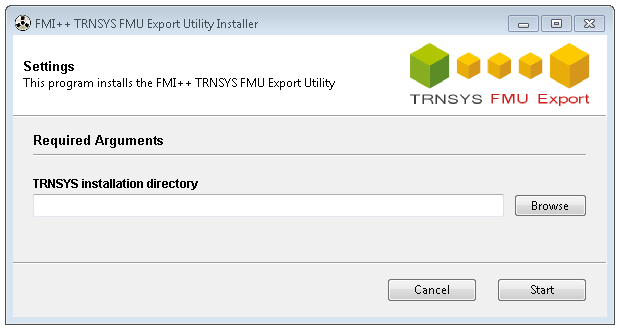
\includegraphics[width=0.98\textwidth]{trnsys_fmu_install_gui}}
\caption{View of the FMI++ TRNSYS FMU Export Utility installer.}
\label{fig:trnsys_fmu_install_gui}
\end{figure}

\begin{figure}[h]
\centering{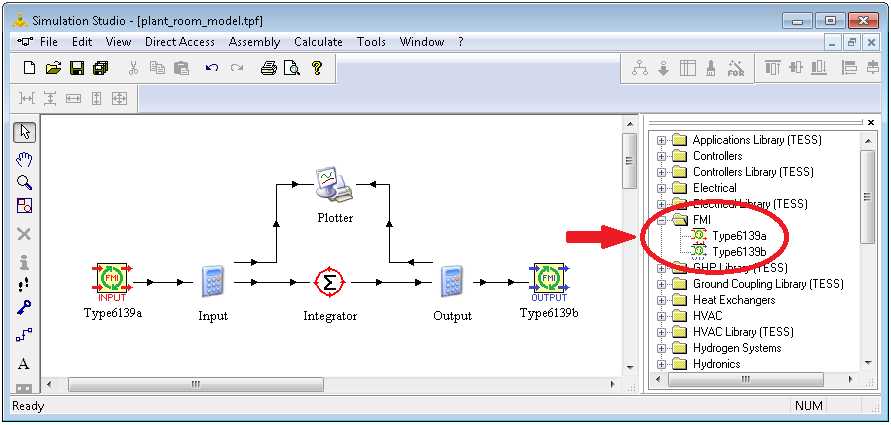
\includegraphics[width=\textwidth]{simulation_studio_overview}}
\caption{Simulation Studio with \type successfully installed.}
\label{fig:simulation_studio_overview}
\end{figure}

